\documentclass[english,onecolumn]{elsarticle}
\usepackage[T1]{fontenc}
\usepackage[utf8]{inputenc}
\usepackage[a4paper]{geometry}
\geometry{verbose}
\usepackage{babel}
\usepackage{amsmath}
\usepackage{amssymb,amsthm}
\usepackage{graphicx}
\usepackage{esint}
\usepackage[unicode=true]
 {hyperref}

\makeatletter

\usepackage{times}
%\usepackage{subfloat}
%\usepackage{subfig}
\usepackage{psfrag}
\usepackage{babel}
\usepackage{times}

\def\d{\mathrm{d}}
\def\dmu{\mathrm{d}\mu}
\def\Esp{\mathbb{E}}
\def\Rset{\mathbb{R}}
\def\X{\mathcal{X}}

\newtheorem{definition}{Definition}
\newtheorem{proposition}{Proposition}

%%%
\makeatletter
\def\ps@pprintTitle{%
  \let\@oddhead\@empty
  \let\@evenhead\@empty
  \def\@oddfoot{\reset@font\hfil\thepage\hfil}
  \let\@evenfoot\@oddfoot
}
\makeatother

\makeatother

\begin{document}

\title{T'aurais pas une entropie?}


\author{by jfb \& co \date}
\begin{abstract}
Where we show that it is possible to derive new entropies yielding
a particular specified maximum entropy distribution. There are (probably)
many errors --I hope not fundamental but is is possible; (certainly
many) approximations, typos, maths and language mistakes.Suggestions
and improvements will be much appreciated. 
\end{abstract}
\maketitle

% -------------------- MaxEnt -------------------- %

\section{Maximum entropy distributions}

Let $f$ be a probability distribution  defined with respect to a general measure
$\mu$ on a set $\X$ and $\displaystyle S[f] = - \int_{\X} f(x) \log f(x)\dmu(x)$
be  the Shannon  entropy of  $f$.   Subject to  $n$ moment  constraints such  as
$\Esp[T_i(x)] = t_i,  i = 1, \ldots,  n$ and to normalization, it  is well known
that the maximum entropy distribution lies within the exponential family
%
\[
f_X(x) = \exp\left(\sum_{i=1}^n \lambda_i T_i(x) + \lambda_0\right).
\]
%
In order  to recover  known probability distributions  (that must belong  to the
exponential family), it is then sufficient  to specify a set of functions $T_i$,
i.e., a  function $T: \Rset \mapsto \Rset^n$  where $n$ is the  number of moment
constraints.   This has  been used  by many  authors.  For  instance,  the gamma
distribution can  be viewed as a  maximum entropy distribution if  one knows the
moments  $\Esp[X]$  and  $\Esp[\log(X)].$  In  order  to  find  maximum  entropy
distributions  with   simpler  constraints  or  distributions   outside  of  the
exponential  family,  it is  possible  to  consider  other entropies,  which  is
discussed below.  This problem find interests in goodness-and-fit tests based on
maximum entropy principle.


% -------------------- Max (h,phi)-Ent -------------------- %

\section{Maximum $(h,\phi)$-entropy distributions}


% ---------- Definition & MaxEnt solutions

\subsection{Definition and maximum $(h,\phi)$-entropy solution}

%\global\long\def\dmu#1{\mathrm{d}\mu(#1)}

\begin{definition}
  Let  $\phi:  \Omega  \subset  \Rset_+  \mapsto  \Rset$  be  a  stricly  convex
  differentiable function defined on a closed convex set $\Omega$.  Then, if $f$
  is  a probability  distribution  defined  with respect  to  a general  measure
  $\mu(x)$ on a set $\X$,
%
\begin{equation}
H_\phi[f] = - \int_{\X} \phi(f(x)) \dmu(x)
\label{eq:phi-entropy}
\end{equation}
%
is the $\phi$-entropy of $f$.
\label{def:phi_entropy}
\end{definition}
%
Since $\phi(x)$ is convex, then the entropy functional $H_{\phi}[f]$ is concave.
Also  note that  the composition  of a  concave function  with a  nondecreasing
concave function preserves concavity, and  that composition of a convex function
with a nonincreasing convex function yields a concave functional.

\begin{definition}%\cite{Sal93,Men97}
%
With the same assumption in definition~\ref{def:phi_entropy},
%
\begin{equation}
H_{h,\phi}[f] = h\left( - \int_{\X} \phi(f(x)) \dmu(x) \right)
\label{eq:h-phi-entropy}
\end{equation}
%
is called $(h,\phi)$-entropy of $f$, where
%
\begin{itemize}
\item either $\phi$ is convex  and $h$ concave  nondecreasing
\item or $\phi$ is concave and $h$ convex nonincreasing
\end{itemize}
\end{definition}
%
These  $(h,\phi)$-entropies  have   been  studied  in~\cite{Sal93,MenMor97}  for
instance. In  these works neither concavity  (resp.\ convexity) of  $h$, nor the
differentiability of $\phi$ are imposed.

A  useful  related  quantity  to  these  entropies  is  the  Bregman  divergence
associated with convex function $\phi$:
%
\begin{definition}
  With  the  same assumption  in  definition~\ref{def:phi_entropy}, the  Bregman
  divergence associated with $\phi$ defined  on a closed convex set $\Omega,$ is
  given by
  %
  \begin{equation}
    D_{\phi}(x_1,x_2)=\phi(x_{1})-\phi(x_{2})-\phi'(x_{2})\left(x_{1}-x_{2}\right).
  \end{equation}
  %
  \label{def:Bregman}
\end{definition}
%
A direct consequence  of the strict convexity of $\phi$  is the nonnegativity of
the Bregman  divergence: $D_\phi(x_1,x_2)  \ge 0$ with  equality if and  only if
$x_1 = x_2$.

\

Consider the  problem of maximizing entropy  \eqref{eq:h-phi-entropy} subject to
constraints  on  some moments  $\Esp\left[T(X)\right]$  where the  normalization
constraint is now included  in $T$ (namely $T_0(x) = 1$ and  $t_0 = 1$). Without
loss of generality,  we consider in the sequel that $\phi$  is convex. Since $h$
is nondecreasing,  it is enough  to look for  the maximum of  the $\phi$-entropy
\eqref{eq:phi-entropy},
%
\begin{equation}
\begin{cases}
\max_f & \displaystyle -\int \phi(f(x))\dmu(x)\\[2mm]
%
\text{s.t. } & \Esp\left[T(X)\right] = t%\\[2mm]
%
\end{cases}
\label{eq:MaxEnt}
\end{equation}
%
\begin{proposition}
  The   probability  distribution   $f_X$  solution   of  the   maximum  entropy
  problem~\eqref{eq:MaxEnt} satisfies the equation
%
\begin{equation}
\phi' \big( f_X(x;t) \big) = \lambda^t \, T(x).
\label{eq:sol-h-phi}
\end{equation}
%
where vector $\lambda$ is such that $\Esp[T(X)] = t$.
\end{proposition}
%
\begin{proof}
%
  The  maximization   problem  being  concave,   the  solution  exists   and  is
  unique.  Equation~\ref{eq:sol-h-phi}  results   directly  from  the  classical
  Lagrange multipliers technique.

An  alternative  derivation  of  the   result  consists  in  checking  that  the
distribution (\ref{eq:sol-h-phi}) is effectively a maximum entropy distribution,
by showing that $H_{\phi}[f]>H_{\phi}[g]$ for all probability distributions with
a  given  (fixed) moment  $\Esp\left[T(X)\right].$  To  this  end, consider  the
functional  Bregman divergence  acting on  functions defined  on a  comon domain
$\X$:
%
\[
D_{\phi}(f_1,f_2) = \int_{\X} \phi(f_1(x)) \dmu(x) - \int_{\X} \phi(f_2(x))
\dmu(x) - \int_{\X} \phi'(f_2(x)) \left( f_1(x) - f_2(x) \right) \dmu(x).
\]
%
From the nonnegativity  of the Bregman divergence this  functional divergence is
nonnegative as well, and zero if and only if $f_1 = f_2$ almost everywhere.
Define by 
%
\[
C_t = \left\{ f: \X \mapsto \Rset_+: \:\: \Esp\left[T(X)\right] = t \right\} 
\]
%
the  set of all  probability distributions  defined on  $\X$ with  given moments
$t$. Consider  now $f_X \in C_t$  such that $\phi'(f_X(x)) =  \lambda^t \, T(x)$
and any given function $f \in C_t$. Then
% 
\begin{eqnarray*}
D_\phi(f,f_X) & = & \int_{\X} \phi(f(x)) \dmu(x) - \int_{\X} \phi(f_X(x))
\dmu(x) - \int_{\X} \phi'(f_X(x)) \left( f(x) - f_X(x) \right) \dmu(x)\\[2mm]
%
& = & - H_\phi[f] + H_\phi[f_X] - \int_{\X} \lambda^t \, T(x) \left( f(x)
- f_X(x) \right) \dmu(x)\\[2mm]
%
& = & H_\phi[f_X] - H_\phi[f]
\end{eqnarray*}
%
where  we   used  the   fact  that   $f$  and  $f_X$   have  the   same  moments
$\Esp\left[T(X)\right]  =  t$.   By   nonegativity  of  the  Bregman  functional
divergence, we finally get that
%
\[
H_\phi[f_X] \ge H_\phi[f]
\]
%
for all pdf $f$ with the same  moments $t$ than $f_X$, with equality if and only
if $f = f_X$ almost everywhere.  In other words, this shows that $f_X$, solution
of (\ref{eq:sol-h-phi}), realizes the minimum of $H_\phi[f]$ over $C_t$.
\end{proof}


% ---------- New entropy functionals

\subsection{Defining new entropy functionals}

Given  an entropy  functional, we  thus obtain  a maximum  entropy distribution.
There exists numerous  $(h,\phi)$-entropies in the literature. However  a few of
them lead to explicit forms for the maximum entropy distribution.  Therefore, it
is  of  high interest  to  look  for the  entropies  that  lead  to a  specified
distribution as a maximum entropy solution. As pointed out previously, this find
interests in goodness-and-fit  tests based in entropies: it  seems convenient to
realize  such  tests  using  the  entropy  such  that  the  distribution  tested
corresponds the its maximum entropy.

Since we will look for the  function $\phi$ for a given probability distribution
$f_X(x)$ we also see that the corresponding $\lambda$ parameters can be included
in the definition of the function.


Let us recall some implicit properties of $\phi(x).$
%
\begin{itemize}
\item $\phi'(x)$ is defined on a domain included on $f_X(\X)$;
%
\item  From the  strict convexity  property  of $\phi$,  necessarily $\phi'$  is
  increasing.
\end{itemize}
%
The identification  of a function  $\phi(x)$ such that  a given $f_X(x)$  is the
associated maximum  entropy distribution amounts  to solve (\ref{eq:sol-h-phi}),
that is
%
\begin{enumerate}
\item choose $T(x)$,
%
\item find $\phi'$ satisfying $\lambda^t T(x) = \phi'(f_X(x))$
%
\item integrate the result to get  $\displaystyle \phi(y) = \int \phi'(y) \d y +
  c$,  where $c$  is  an integration  constant.   The entropy  being defined  by
  $\displaystyle H_\phi[f]  = - \int_{\X} \phi(f(x)) \dmu(x)$,  the constant $c$
  will usually be zero.
% 
\item Parameters $\lambda$ may be choosen  case by case in order to simplify the
  expression of $\phi.$
\end{enumerate}

Remind that $\phi'$  must be increasing, thus, necessarily,  $\lambda^t \, T(x)$
and $f_X(x)$ must have the same sense of variation. Moreover, at a first glance,
eq.~\eqref{eq:sol-h-phi} requires  $f_X$ and  $\lambda^t T(x)$ sharing  the same
symmetries.  Namely,  if  for  two  different  values  $x_1,  x_2  \in  \X$  the
distribution  satisfies  $f_X(x_1)  =  f_X(x_2)$  then $\lambda^t  \,  T(x_1)  =
\lambda^t  \,  T(x_2)$  (this does  mean  that  $T(x_1)$  and $T(x_2)$  must  be
equals). Thus, eq.~\eqref{eq:sol-h-phi} rewrites
%
\begin{equation}
\phi'(y) = \lambda^t T(f_X^{-1}(y))
\label{eq:derivative-phi}
\end{equation}
%
where $f_X^{-1}$ can  be multivalued; in such a  situation, $\phi'$ remains well
defined. Note again that for given $T$ and $f_X$, the solution is not unique due
to  parameters $\lambda$,  which can  be  chosen finely  so as  to simplify  the
expression of $\phi'$. Eq.~\eqref{eq:derivative-phi}  can then be integrated, at
least  formaly, to  achieve $H_\phi$  (and  thus any  $H_{h,\phi}$ entropy  with
nondecreasing $h$).

For instance, for one moment constraint, if $\lambda_1$ is negative, then
%
\begin{itemize}
\item for $T_1(x) = x,$ $f_X(x)$ must be decreasing, %non increasing,
\item for $T_1(x) = x^2$ or $T_1(x) = |x|,$ $f_{X}(x)$ must be unimodal with
a maximum at zero. 
\end{itemize}

%Equation~\eqref{eq:sol-h-phi} may have no solution, when $\lambda^t \, T(x)$ has
%not the same variations than $f_X$. But it can also have several solutions.


% -------------------- Fisher -------------------- %

\section{$\phi$-escort, $\phi$-Fisher information and generalized Cram\'er-Rao inequality}


% -------------------- Examples -------------------- %

\section{Some examples}


% ---------- Normal

\subsection{Normal distribution and second-order moment}

For a normal distribution, and second order moment constraint
%
\[
f_X(x) = \frac{1}{\sqrt{2 \pi} \, \sigma} \exp\left( - \frac{x^2}{2 \, \sigma^2}
\right) \qquad \mbox{and} \qquad \lambda^t T(x) = \lambda_0 + \lambda_1 x^2
\]
%
We begin  by computing the  inverse of  $y = f_X(x)$  where $x \in  \Rset_+$ for
instance,  which   gives
%
\[
\phi'(y) = \left( \lambda_0 - \sigma^2 \log(2 \pi \sigma^2) \, \lambda_1 \right)
- 2 \sigma^2 \lambda_1 \log y
\]
%
The judicious choice
%
\[
\lambda_0 = 1 - \log(\sqrt{2 \pi} \sigma) \qquad \mbox{and} \qquad \lambda_1 = -
\, \frac{1}{2 \, \sigma^2}
\]
%
leads to function
%
\[
\phi(y) = y \log y
\]
%
that gives nothing more than the Shannon entropy as expected.

% ---------- q-Normal

\subsection{$q$-Normal distribution and second-order moment}

For $q$-normal distribution,  also known as Tsallis distributions,  and a second
order moment constraint,
%
\[
f_X(x) = C_q \Big( 1 - (q-1) \beta x^2 \Big)_{\!+}^{\frac{1}{(q-1)}} \qquad
\mbox{and} \qquad \lambda^t T(x) = \lambda_0 + \lambda_1 x^2
\]
%
where $q > 0$ and $x_+ = \max(x,0)$ we get
%
\[
\phi'(y) = \left( \lambda_0 + \frac{\lambda_1}{(q-1) \beta} \right) -
\frac{\lambda_1 \, y^{q-1}}{C_q^{q-1} (q-1) \beta}
\]
%
In this case, a judicious choise of parameters is
%
\[
\lambda_0 = \frac{q \, C_q^{q-1}}{(q-1) \beta} \qquad \mbox{and} \qquad \lambda_1 =
- q \, C_q^{q-1} \beta
\]
%
that yields to
\[
\phi(y) = \frac{y^q}{q-1}.
\]
%
and an associated entropy can be 
\[
H_{h,\phi}[f]=\frac{1}{1-q}\left(\int_{\X} f(x)^q \dmu(x) - 1 \right),
\]
%
which is nothing but Tsallis entropy.
% \footnote{Another possibility should be to  arrive at $\phi(y) = y^q$, that is
%   concave when $q < 1$: by chosing $h(x) = \frac{\log x}{1-q}$}.  \footnote{Of
%   course, we  can also  take the first  $\phi(y)=\frac{y^{q}}{1-q},$ integrate
%   and add any constant, since adding a constant do not modify the actual value
%   af the minimizer (or maximizer if we consider concave entropies).

% ---------- q-exponential

\subsection{$q$-exponential distribution and first-order moment}


% ---------- q-Normal

\subsection{Hyperbolic secant distribution and first-order moment}


Let us consider some specific cases. 
\begin{enumerate}
\item For a normal distribution, $f_{X}(x)=\frac{1}{\sqrt{2\pi}}\exp(-\frac{x^{2}}{2})$
and $T(x)=x^{2},$ we begin by computing the inverse $y=\frac{1}{\sqrt{2\pi}}\exp(-\frac{x^{2}}{2})$,
which gives $-\frac{1}{2}x^{2}-\log\sqrt{2\pi}=\log(y).$ Choosing
$\lambda=-\frac{1}{2}$, $\mu=-\log\sqrt{2\pi}$ and integrating,
we obtain 
\[
\phi(y)=y\log y-y
\]

\item For a Tsallis $q$-exponential, $f_{X}(x)=C_{q}\left(1-(q-1)\beta x\right)_{+}^{\frac{1}{(q-1)}},$
$x\geq0,$ and $T(x)=x$. We simply have $C_{q}^{q-1}\left(1-(q-1)\beta x\right)=y^{q-1}$.
With $\lambda=qC_{q}^{q-1}\beta$ and $\mu=qC_{q}^{q-1}/(1-q)$, this
yields 
\[
\phi(y)=\frac{y^{q}}{1-q}.
\]
Taking $\mu=\left(qC_{q}^{q-1}+1\right)/(1-q)$ gives 
\[
\phi(y)=\frac{y^{q}-y}{1-q},
\]
and an associated entropy can be 
\[
H_{\phi}[f]=\frac{1}{1-q}\left(\int f(x)^{q}\text{d}\mu(x)-1\right),
\]
which is nothing but Tsallis entropy.%
\footnote{Of course, we can also take the first $\phi(y)=\frac{y^{q}}{1-q},$
integrate and add any constant, since adding a constant do not modify
the actual value af the minimizer (or maximizer if we consider concave
entropies). %
}
\item The same entropy functional can readily be obtained for the so-called
$q$-Gaussian, or Student-t and -r distributions $f_{X}(x)=C_{q}\left(1-(q-1)\beta x^{2}\right)_{+}^{\frac{1}{(q-1)}}.$
It suffices to follow the very same steps as above with $T(x)=x^{2}.$ 
\item Let $f_{X}(x)$ be the hyperbolic secant distribution, with density
\[
f_{X}(x)=\frac{1}{2}\text{sech}(\frac{\pi}{2}x)=\frac{1}{2}\cosh^{-1}(\frac{\pi}{2}x).
\]
Obviously, $\frac{\pi}{2}x=\cosh(2y)=\phi'(y)$ with $T(x)=x$, $\lambda=\frac{\pi}{2}$,
and 
\[
\phi(y)=\sinh(2y).
\]
So doing, we obtain an hyperbolic sine entropy with the hyperbolic
secant distribution as the associated maximum entropy distribution.
\end{enumerate}
Of course, the preceeding derivations require that (\ref{eq:inv})
is effectively solvable. Furthermore, one has also to choose or design
a specific $T(x)$ statistic, as well as the parameters $\lambda$
and $\mu$. In the examples above, we used $T(x)=x$ and $T(x)=x^{2}.$
Particular choices such as $T(x)=x^{2}$ or $T(x)=|x|$ obviously
lead to symmetrical densities. The case of nonsymmetrical unimodal
densities seems to be much more involved. For instance, if we take
$T(x)=x$, then the resolution of (\ref{eq:inv}) amounts to compute
the inverse relation of $f_{X}(x)$, which is is multi-valued. We
will deal now with this special case. 


\subsection{Entropies for unimodal nonsymmetric distributions}

Assume, without loss of generality that the mode is $x=0.$ Let $T(x)=x$,
and $\lambda=-1$, $\mu=0.$ In such case, we have to find $\phi$
satisfying $x=-\phi'\left(f_{X}(x)\right)=-\phi'(y)$. We see that
$\phi'$ is minus the inverse relation of $y=f_{X}(x)$. But $f_{X}(x)$
is not injective and to each $y$ correspond a positive and a negative
value of $x.$ Hence we have two partial inverses, say $\phi_{+}'$
and $\phi_{-}'$ such that $\phi_{+}'^{-1}(-x)=f_{X}(x)$ for $x\geq0$
and $\phi_{-}'^{-1}(-x)=f_{X}(x)$ for $x\leq0$. We observed above
that if $f_{X}(x)$ is non increasing, that is assumed here for $x\geq0,$
then $\phi_{+}''\geq0$ and $\phi_{+}$is convex. Then, our proposal
is to use the functional $\phi_{+}$ for defining a $\phi$-entropy
\[
H_{\phi}[f_{X}]=\int\phi_{+}\left(f_{X}(x)\right)\dmu x
\]
associated with a specific nonsymmetric probability distribution.
In this setting, it is understood that the maximum entropy distribution
$f_{X}(x)=\phi'^{-1}(-x)$ will have to be computed as $\phi_{+}'^{-1}(-x)=f_{X}(x)$
for $x\geq0$ and $\phi_{-}'^{-1}(-x)=f_{X}(x)$ for $x\leq0$. Of
course, this does not forbid to model one-sided probability distribution,
provided that the constraint is included in the formulation of the
maximum entropy problem. 


\subsubsection{Example 1. The logistic distribution}

The pdf of the logistic distribution is given by
\[
f_{X}(x)=\frac{e^{-\frac{x}{s}}}{s\left(1+e^{-\frac{x}{s}}\right)^{2}}.
\]
This distribution, which resembles the normal distribution but has
heavier tails, has been used in many applications. By direct calculations,
we obtain 
\[
\begin{cases}
\phi_{-}'(y)= & s\ln\left(\frac{1}{2}\,{\frac{-2\, ys+1+\sqrt{-4\, ys+1}}{ys}}\right),\\
\phi_{+}'(y)= & s\ln\left(-\frac{1}{2}\,{\frac{2\, ys-1+\sqrt{-4\, ys+1}}{ys}}\right).
\end{cases}
\]


The associated entropy is then 
\[
\phi_{+}(y)=\frac{1}{2}\,\sqrt{-4\, ys+1}+ys\,\ln\left(-{\frac{\sqrt{-4\, ys+1}-1}{\sqrt{-4\, ys+1}+1}}\right),
\]
for $y\in[0,\frac{1}{4s}],$ and where we have introduced a integration
constant such that $\min_{y}\phi_{+}(y)=0.$ For $y>\frac{1}{4s},$
we extend the function and let $\phi_{+}(y)=+\infty.$ Figure \ref{fig:Entropy-logistic}
\begin{figure}
%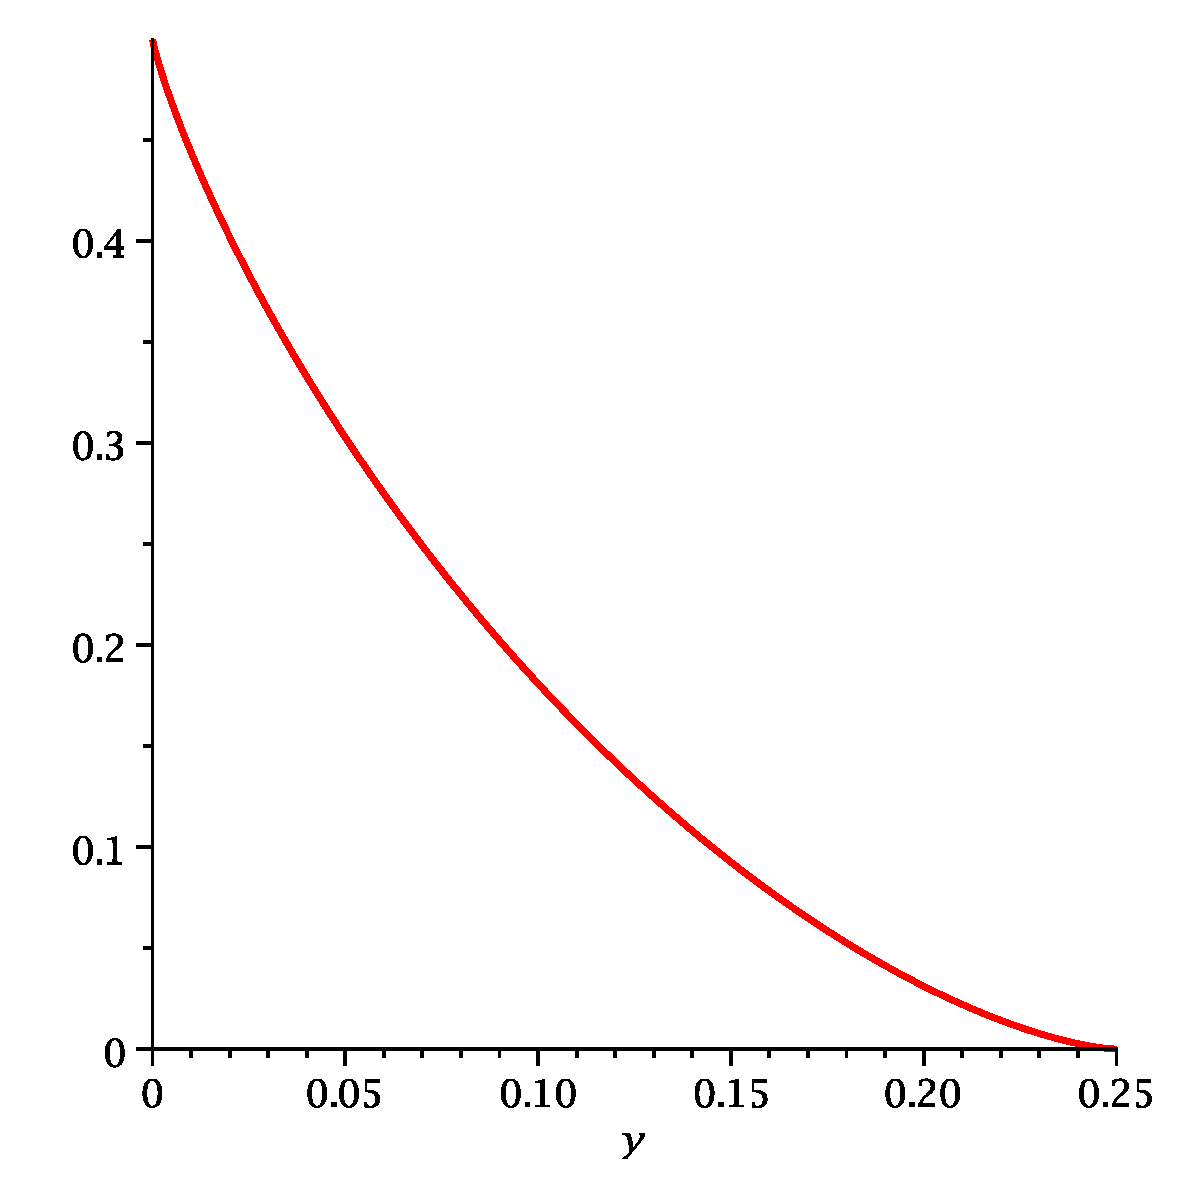
\includegraphics[width=5cm]{maple/phi_logistic}\caption{Entropy derived from the logistic distribution. \label{fig:Entropy-logistic}}
\end{figure}
gives a representation of this entropy for $s=1.$ 


\subsubsection{Example 2. The gamma distribution}

The probability density function of the gamma distribution is given
by 
\[
f_{X}(x)=\frac{{\beta}^{\alpha}{x}^{\alpha-1}{e}^{-\beta\, x}}{\Gamma\left(\alpha\right)}
\]


We obtain 
\[
\phi'(y)=-{{\rm e}^{\frac{1}{\alpha-1}\left(-{\it W}\left(-{\frac{\beta\,\left(y\Gamma\left(\alpha\right){\beta}^{-\alpha}\right)^{\left(\alpha-1\right)^{-1}}}{\alpha-1}}\right)\alpha+{\it W}\left(-{\frac{\beta\,\left(y\Gamma\left(\alpha\right){\beta}^{-\alpha}\right)^{\left(\alpha-1\right)^{-1}}}{\alpha-1}}\right)+\ln\left(y\Gamma\left(\alpha\right){\beta}^{-\alpha}\right)\right)}},
\]
where ${\it W}$ is the Lambert W multivalued `function' defined by
$z=W(z)e^{W(z)}$ (ie the inverse relation of $f(w)=we^{w}$). Unfortunately,
in the general case, we do not have a closed form for $\phi(y)$ as
the integral of $\phi'(y)$.%
\footnote{This might not be completely unacceptable. Indeed, it is really not
difficult to compute numerically the values of $\phi(y).$%
} Restricting us to the case $\alpha=2$, we have
\[
\phi(y)=\frac{\left(1-{\it W}\left(-{\frac{y}{\beta}}\right)+y\left({\it W}\left(-{\frac{y}{\beta}}\right)\right)^{2}\right)}{{\it \beta\, W}\left(-{\frac{y}{\beta}}\right)}+\frac{\beta}{e},
\]
which is convex if we choose the -1 branch of the Lambert function.
An example with $\alpha=2$ and $\beta=3$ is given on Figure \ref{fig:Entropy-gamma}.
\begin{figure}
%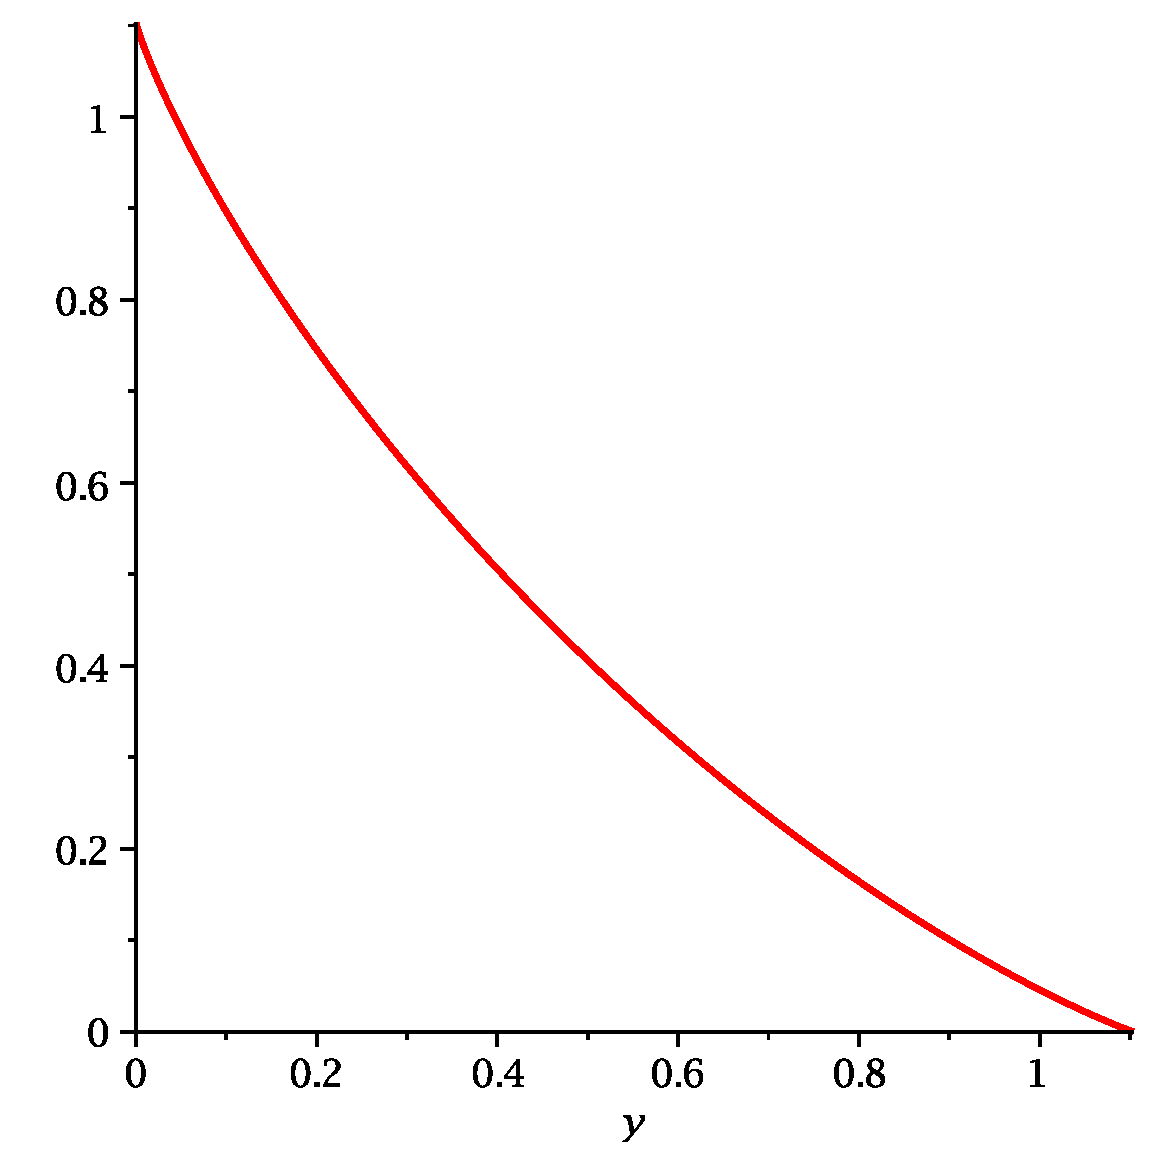
\includegraphics[width=5cm]{maple/phi_gamma}\caption{\label{fig:Entropy-gamma}Entropy derived from the gamma distribution}
\end{figure}



\subsubsection{Example 3. The arcsine distribution}

As a last example, and though it is not a unimodal density (! but
yields the same problem for inversion), let us consider the case of
the arcsine distribution (see \href{http://en.wikipedia.org/wiki/Arcsine_distribution}{wiki}).
This distribution, defined for $x\in(0,1),$ is a special case of
the Beta distribution with parameters $\alpha=\beta=1/2.$ It has
the following pdf:
\[
f_{X}(x)=\frac{1}{\pi\sqrt{x(1-x)}}.
\]
Observe that $\min_{x}f_{X}(x)=2/\pi.$ Doing our now usual calculations,
we obtain
\[
\begin{cases}
\phi_{-}'(y)= & -\frac{\, y\pi+\,\sqrt{{y}^{2}{\pi}^{2}-4}}{2y\pi},\\
\phi_{+}'(y)= & -\frac{\, y\pi-\,\sqrt{{y}^{2}{\pi}^{2}-4}}{2y\pi}.
\end{cases}
\]
and the expression of the entropy is 
\[
\phi_{+}(y)=\frac{1}{2}\,{\frac{\sqrt{{y}^{2}{\pi}^{2}-4}}{\pi}}+\frac{1}{\pi}\arctan\left(2\,{\frac{1}{\sqrt{{y}^{2}{\pi}^{2}-4}}}\right)-\frac{1}{2}\, y,
\]
for $y\geq1/\pi$. The entropy is shown on Figure \ref{fig:arcseine entropy}.
\begin{figure}
%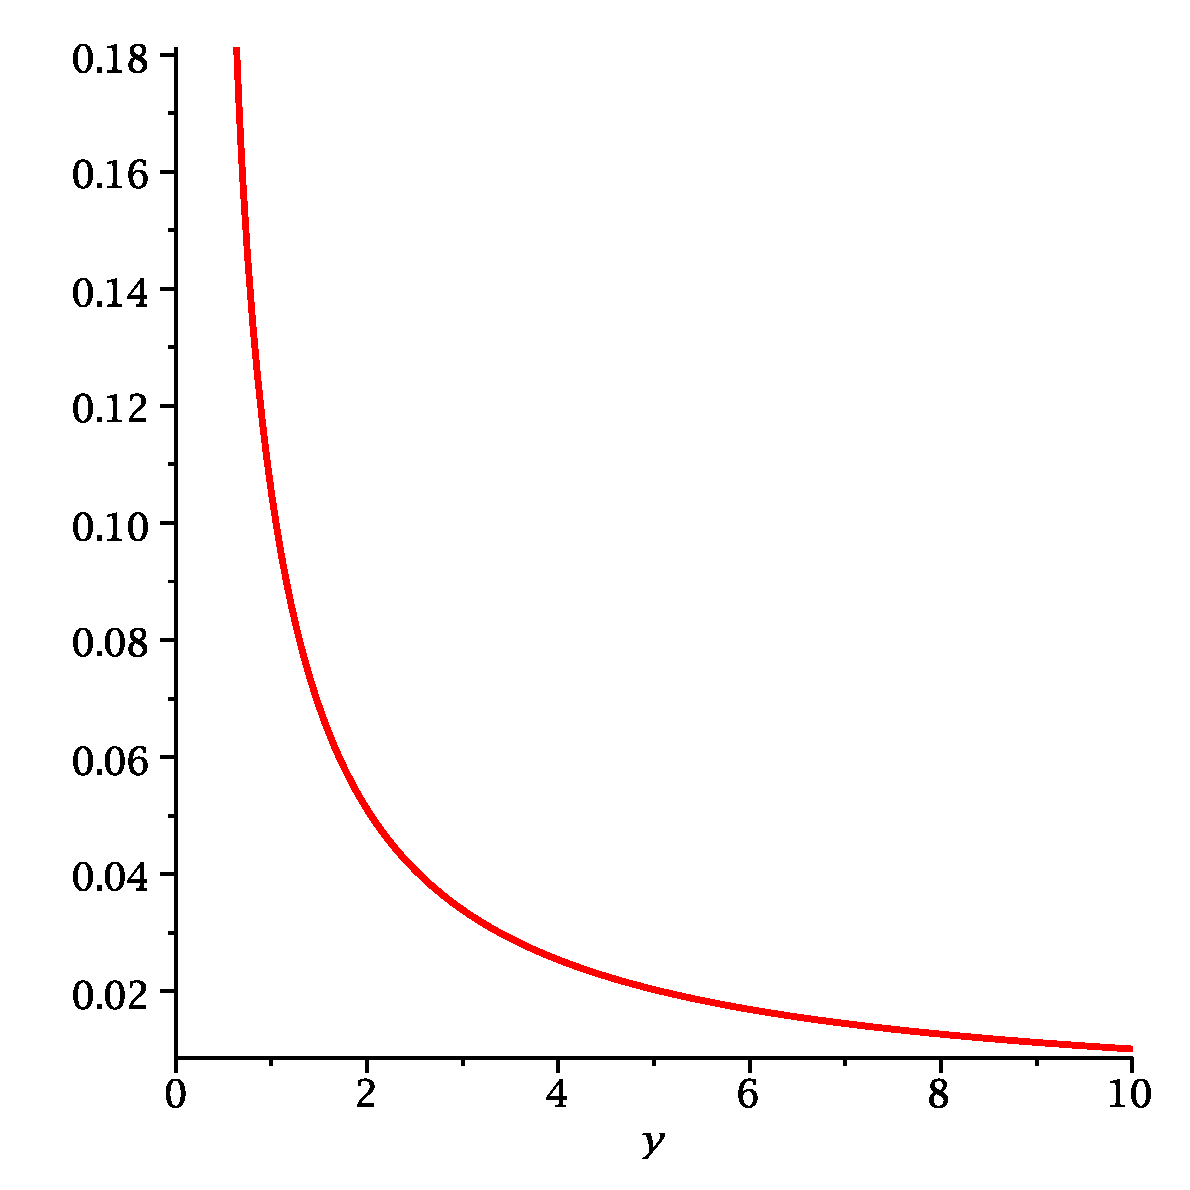
\includegraphics[width=5cm]{maple/phi_arcsine}\caption{The entropy associated with an arcsine distribution. \label{fig:arcseine entropy}}
\end{figure}

\end{document}
